%%%%%%%%%%%%%%%%%%%%%%%%%%%%%%%%%%%%%%%%%
% Beamer Presentation
% LaTeX Template
% Version 1.0 (10/11/12)
%
% This template has been downloaded from:
% http://www.LaTeXTemplates.com
%
% License:
% CC BY-NC-SA 3.0 (http://creativecommons.org/licenses/by-nc-sa/3.0/)
%
%%%%%%%%%%%%%%%%%%%%%%%%%%%%%%%%%%%%%%%%%
% Presentation - 	Kushal Khandelwal
% Master Thesis : 	Automatic Methods for Vessel Segmentation in Fundus Images
% Submitted : 		8 May 2015
%----------------------------------------------------------------------------------------
%	PACKAGES AND THEMES
%----------------------------------------------------------------------------------------

\documentclass{beamer}

\mode<presentation> {
	
	% The Beamer class comes with a number of default slide themes
	% which change the colors and layouts of slides. Below this is a list
	% of all the themes, uncomment each in turn to see what they look like.
	
	%\usetheme{default}
	%\usetheme{AnnArbor}
	%\usetheme{Antibes}
	%\usetheme{Bergen}
	%\usetheme{Berkeley}
	%\usetheme{Berlin}
	%\usetheme{Boadilla}
	\usetheme{CambridgeUS}
	%\usetheme{Copenhagen}
	%\usetheme{Darmstadt}
	%\usetheme{Dresden}
	%\usetheme{Frankfurt}
	%\usetheme{Goettingen}
	%\usetheme{Hannover}
	%\usetheme{Ilmenau}
	%\usetheme{JuanLesPins}
	%\usetheme{Luebeck}
	%\usetheme{Madrid}
	%\usetheme{Malmoe}
	%\usetheme{Marburg}
	%\usetheme{Montpellier}
	%\usetheme{PaloAlto}
	%\usetheme{Pittsburgh}
	%\usetheme{Rochester}
	%\usetheme{Singapore}
	%\usetheme{Szeged}
	%\usetheme{Warsaw}
	
	% As well as themes, the Beamer class has a number of color themes
	% for any slide theme. Uncomment each of these in turn to see how it
	% changes the colors of your current slide theme.
	
	%\usecolortheme{albatross}
	%\usecolortheme{beaver}
	%\usecolortheme{beetle}
	%\usecolortheme{crane}
	%\usecolortheme{dolphin}
	%\usecolortheme{dove}
	%\usecolortheme{fly}
	%\usecolortheme{lily}
	%\usecolortheme{orchid}
	\usecolortheme{rose}
	%\usecolortheme{seagull}
	%\usecolortheme{seahorse}
	%\usecolortheme{whale}
	%\usecolortheme{wolverine}
	
	%\setbeamertemplate{footline} % To remove the footer line in all slides uncomment this line
	%\setbeamertemplate{footline}[page number] % To replace the footer line in all slides with a simple slide count uncomment this line
	
	%\setbeamertemplate{navigation symbols}{} % To remove the navigation symbols from the bottom of all slides uncomment this line
}

\usepackage{graphicx} % Allows including images
\usepackage{booktabs} % Allows the use of \toprule, \midrule and \bottomrule in tables

%----------------------------------------------------------------------------------------
%	TITLE PAGE
%----------------------------------------------------------------------------------------

\title[Vessel Segmentation Methods]{Automatic Methods for Vessel Segmentation\\ in \\Fundus Images} % The short title appears at the bottom of every slide, the full title is only on the title page

\author{Kushal Khandelwal} % Your name
\institute[HCI] % Your institution as it will appear on the bottom of every slide, may be shorthand to save space
{
	Heidelberg Collaboratory for Image Processing \\ % Your institution for the title page
	\medskip
	\textit{kushal.khandelwal@iwr.uni-heidelberg.de} % Your email address
}
\date{\today} % Date, can be changed to a custom date

\begin{document}
	
	\begin{frame}
		\titlepage % Print the title page as the first slide
	\end{frame}
	
	\begin{frame}
		\frametitle{Overview} % Table of contents slide, comment this block out to remove it
		\tableofcontents % Throughout your presentation, if you choose to use \section{} and \subsection{} commands, these will automatically be printed on this slide as an overview of your presentation
	\end{frame}
	
	%----------------------------------------------------------------------------------------
	%	PRESENTATION SLIDES
	%----------------------------------------------------------------------------------------
	
	%------------------------------------------------
	\section{Introduction} % Sections can be created in order to organize your presentation into discrete blocks, all sections and subsections are automatically printed in the table of contents as an overview of the talk
	%------------------------------------------------
	
	\subsection{Objective} % A subsection can be created just before a set of slides with a common theme to further break down your presentation into chunks
	
		\begin{frame}
			\frametitle{Retinal Vessel Segmentation}
			
			\begin{columns}[c] % The "c" option specifies centered vertical alignment while the "t" option is used for top vertical alignment
				
				\column{.45\textwidth} % Left column and width
				
				Automatic methods for Retinal Vessel Segmentaion in Fundus Images
				
				\column{.5\textwidth} % Right column and width
				\begin{figure}
					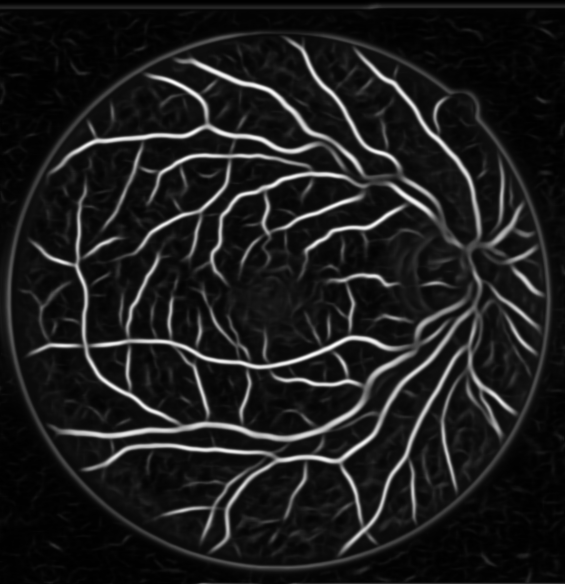
\includegraphics[width=0.6\linewidth]{Images/slide1.png}
				\end{figure}
				
			\end{columns}
		\end{frame}
	%------------------------------------------------
	
	\begin{frame}
		\frametitle{Task}
		\begin{figure}
			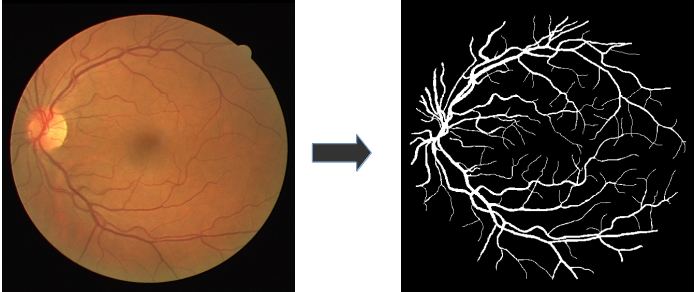
\includegraphics[width=1.0\linewidth]{Images/Graphic1.png}
		\end{figure}
	\end{frame}
	
	%------------------------------------------------
	\subsection{Challenges}
	\begin{frame}
		\frametitle{Challenges and Limitations}
		\begin{block}{}
			\begin{itemize}
				\item False vessel detections
				\item Varying vessel width
				\item Merging of close vessels
				\item Bifurcation of vessels
				\item Merging of close vessels
				\item Presence of other structures like hemorrhage spots, exudates and lesions.
			\end{itemize}
	\end{block}
	\end{frame}
	
	%------------------------------------------------
		\begin{frame}
			\frametitle{Challenges}
				\begin{figure}
					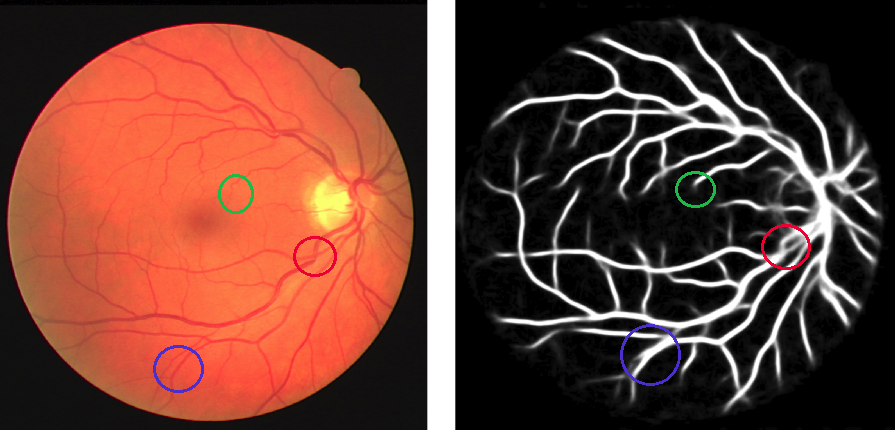
\includegraphics[width=1.0\linewidth]{Images/problem1.png}% Insert Image with cropping
					\caption{In blue, merging of close vessels, in red poor segmentation at crossover, and in green, poor segmentation of thin vessels}
				\end{figure}
		\end{frame}
	%------------------------------------------------


	%------------------------------------------------
	\section{Literature Review}
	%------------------------------------------------
			\begin{frame}
				\frametitle{Related Work}
				\begin{figure}
					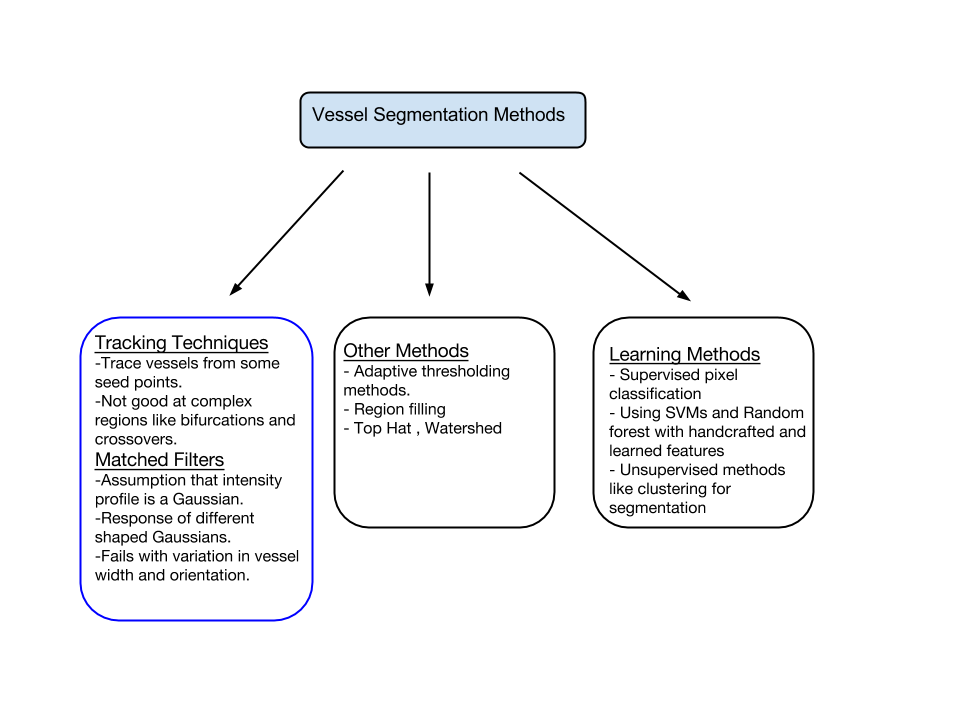
\includegraphics[width=0.9\linewidth]{methods/m1.png}% Insert Image with cropping
				\end{figure}
			\end{frame}
			
			\begin{frame}
				\frametitle{Related Work}
				\begin{figure}
					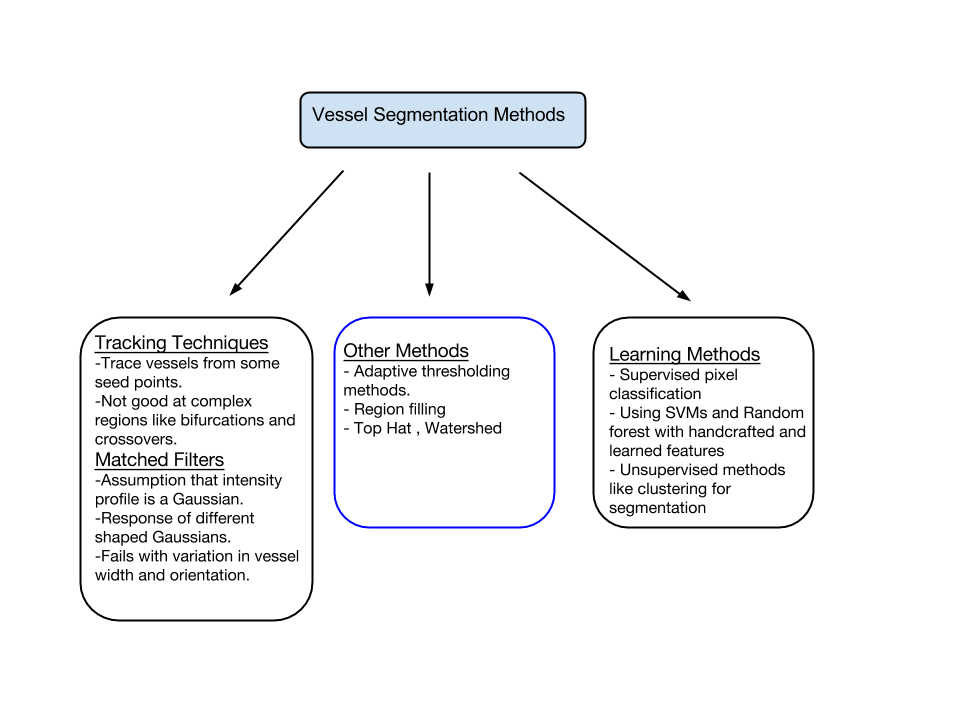
\includegraphics[width=0.9\linewidth]{methods/m2.png}% Insert Image with cropping
				\end{figure}
			\end{frame}
			
			\begin{frame}
				\frametitle{Related Work}
				\begin{figure}
					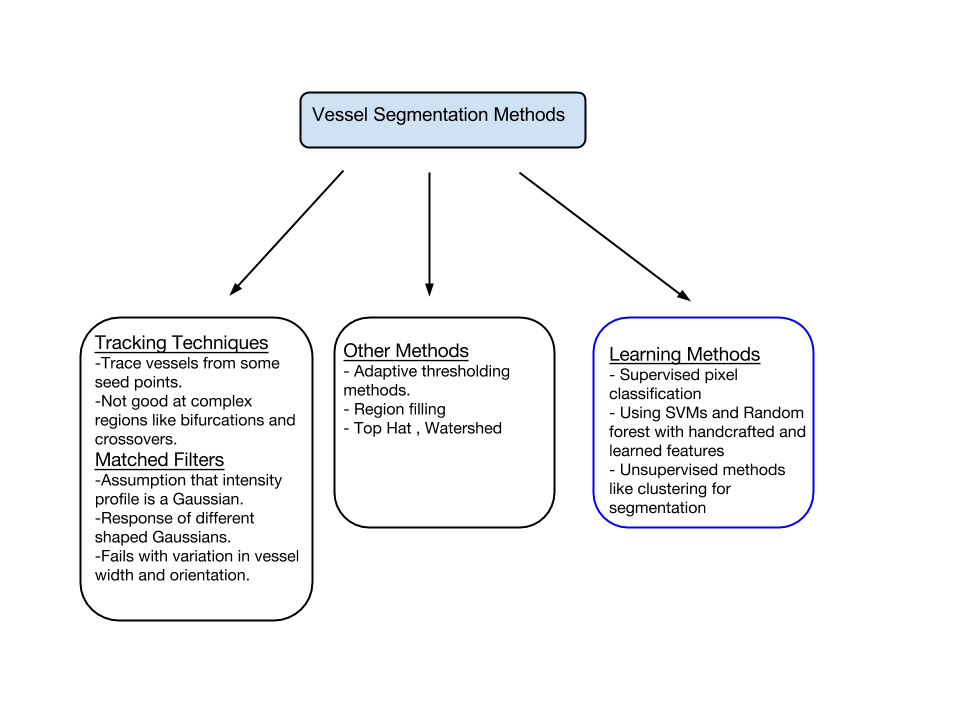
\includegraphics[width=0.9\linewidth]{methods/m3.png}% Insert Image with cropping
				\end{figure}
			\end{frame}
%	\begin{frame}
%		\frametitle{Related Work}
%		There has been a lot of work on retinal image segmentation. Some of them are :
%		\begin{itemize}
%			\item Tracking techniques to trace vessels starting from some seed points.
%			
%			\item Mathematical morphology based techniques.
%			\item Model based approaches 
%			\item Staal et al, presented a ridge based vessel segmentation methods.
%			\item Ricci and Perfetti proposed a methodology using line operators as feature vectors and SVM for pixel classification.
%			\item Osareh and Shadgar used multiscale Gabor filters for vessel candidate identification.
%			\item Supervised pixel classification methods.
%		\end{itemize}
%	\end{frame}
	%------------------------------------------------
	\begin{frame}
		\frametitle{Related Work}
		Now, we talk about four of the recent advancements in the vessel segmentation methods, to have a comparison with our approach
		\begin{itemize}
			
			\item Structured Forests for Fast Edge Detection (SE) [Dollar et al]
			\item Accurate and Efficient Linear Structure Segmentation by leveraging Ad Hoc Features with learned Filters (CS) [Rigamonti et al]
			\item Filter Learning for Linear Structure Segmentation (DL) [R.Rigamonti]
			\item Neural Network Nearest Neighbor Fields for Image Transforms (N4) [Ganin et al]
		\end{itemize}
		
	\end{frame}
	
	%------------------------------------------------------%

	
	\begin{frame}
		\frametitle{Structured Forests}

			\begin{itemize}
				\item Exploits the presenece of structures like edges, T-junctions in small local image patches.
				\item Trains structured forests over these local image patches and their segmentation maps. 
				\item Learns multiple edge maps, which are aggregated to obtain final edge map.
			\end{itemize}
		
	\end{frame}
	\begin{frame}
		\frametitle{Structured Forests}
		\begin{figure}
			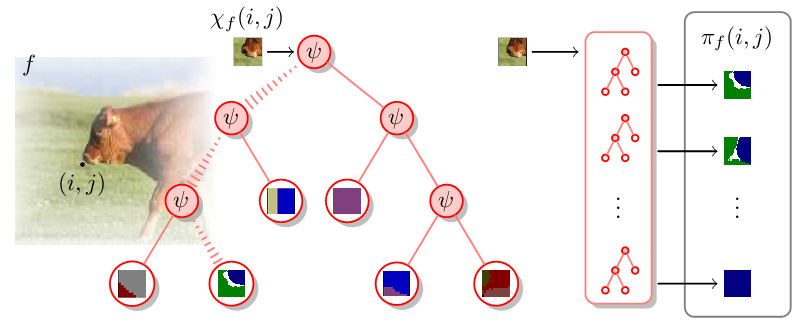
\includegraphics[width=\linewidth]{methods/se.png}
			\caption{An example of Structured Random forests for image segmentation (https://pdollar.wordpress.com/2013/03/08/structured-random-forests/)}
		\end{figure}

	\end{frame}
	
	
	%------------------------------------------------------%
	\begin{frame}
		\frametitle{Filter Learning for Linear Structure Segmentation}

			\begin{itemize}
				\item Learns a filter bank from a set of representative training images in a sparse convolution coding way.
				\item Features maps are computed by convolving the filters with the images.
				\item A random forest classifier is trained to classify each image location as lying on a linear structure or background.
			\end{itemize}			
	\end{frame}
	\begin{frame}
			\begin{figure}
				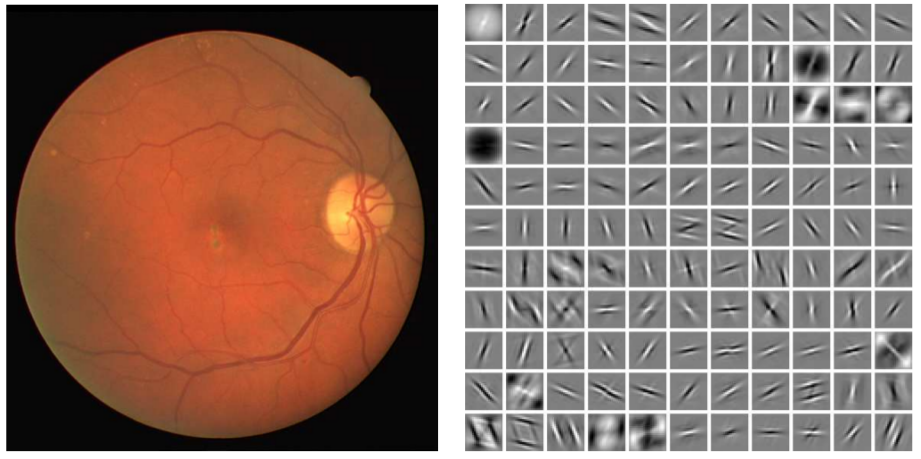
\includegraphics[width=0.6\linewidth]{methods/dl.png}
			\end{figure}			
	
	\end{frame}
	
		
		
		
		%------------------------------------------------------%

	\begin{frame}
		\frametitle{Ad Hoc Features and Learned Filters}
			\begin{itemize}
				\item Linear filters are learned by modeling the distribution of image representatives.
				\item Filters are learned in a convolutional sparse learning model.
				\item Features maps are computed using the learned filters and other hand crafted features  are computed.
				\item A random forest classifier is trained to classify each image location as lying on a linear structure or background.
			\end{itemize}			

	\end{frame}
	

	%------------------------------------------------------%
	

	

	%------------------------------------------------------%
	

	
	\begin{frame}
		\frametitle{Neural Network Nearest Neighbor Fields for Image Transforms}

			\begin{figure}
				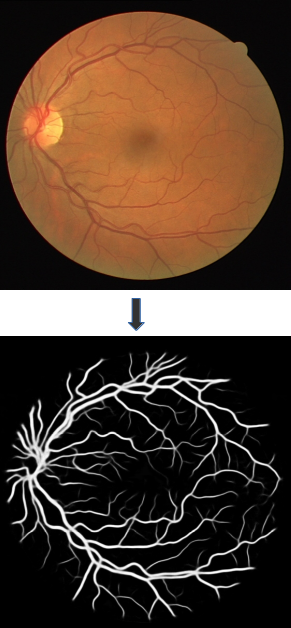
\includegraphics[width=0.6\linewidth]{Images/N4.png}
			\end{figure}
			

			\begin{itemize}
				\item CNN is trained to learn an intermediate mapping for the patches. Each patch is mapped to an intermediate annotation map.
				\item For a given set of intermediate mapping of training patches, a dictionary is learned mapping to the GT patches.
				\item New input patches are assigned annotation from the dictionary patch with the closest CNN output.
			\end{itemize}					
	
	\end{frame}

	%------------------------------------------------
	\section{Framework}
	%------------------------------------------------	
	\begin{frame}
		\frametitle{Architecture}
		\begin{itemize}
			\item We approach the problem in a patch based framework
			\item In a patch based framework, we extract patches around each pixel taken at centre, and make individual predictions for each patch.
			\item Using image patches and their corresponding segmentation masks, we learn a dictionary of individual patches mapped to the segmentation masks.
			\item This learned dictionary is then used to make predictions by matching the new patches to the dictionary.
			\item Segmentation map is reconstructred from the patches.
		\end{itemize}
	\end{frame}
	
	\begin{frame}
		\frametitle{Architecture}
			\begin{figure}
				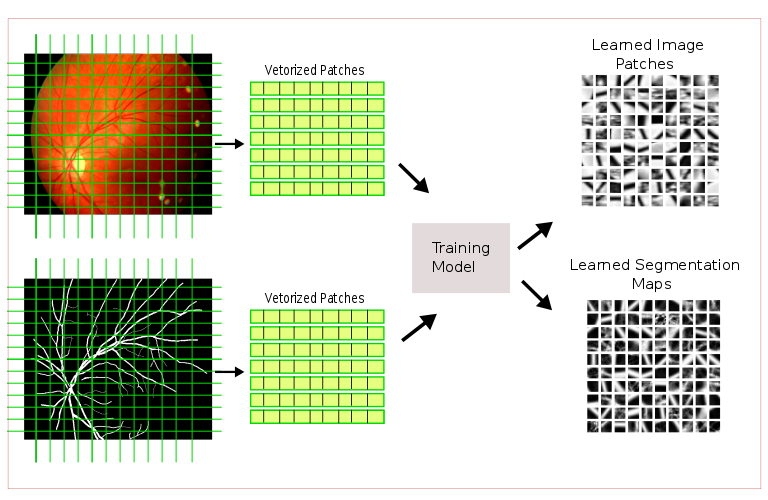
\includegraphics[width=1\linewidth]{framework/trainmodel.png}
			\end{figure}
	\end{frame}
	
	\begin{frame}
		\frametitle{Architecture}
		We propose two different models to learn these dictionaries:
		\begin{itemize}
			\item k-means clustering model for local structure dictionary learning.
			\item Sparse Coding dictionary of local structures.
		\end{itemize}
	\end{frame}
	
	%------------------------------------------------
	\section{Models}
	%------------------------------------------------	
	\subsection{Clustering Model}
	\begin{frame}[t]
		\frametitle{Clustering Model}
		\begin{itemize}
			\item Learn local structures like edges and straight lines.
	
		\end{itemize}
	\end{frame}
	\begin{frame}[t]
		\frametitle{Clustering Model}
		\begin{itemize}
			\item Learn local structures like edges and straight lines.
			\item Image patches are clustered using K-means to find common local structures withing all the image patches.

		\end{itemize}
	\end{frame}	
	\begin{frame}[t]
		\frametitle{Clustering Model}
		\begin{itemize}
			\item Learn local structures like edges and straight lines.
			\item Image patches are clustered using K-means to find common local structures withing all the image patches.
			\item Each of these clusters are assigned segmentation maps, obtained by averaging the segmentation maps of all the patches within a cluster.

		\end{itemize}
	\end{frame}	
	\begin{frame}[t]
		\frametitle{Clustering Model}
		\begin{itemize}
			\item Learn local structures like edges and straight lines.
			\item Image patches are clustered using K-means to find common local structures withing all the image patches.
			\item Each of these clusters are assigned segmentation maps, obtained by averaging the segmentation maps of all the patches within a cluster.
			\item A dictionary is made of these clustered structures and segmentation maps.
		\end{itemize}
	\end{frame}	
	
	\begin{frame}{Dictionary using Clustering model}
			\begin{columns}[c] % The "c" option specifies centered vertical alignment while the "t" option is used for top vertical alignment
				
				\column{.45\textwidth} % Right column and width
					\begin{figure}
						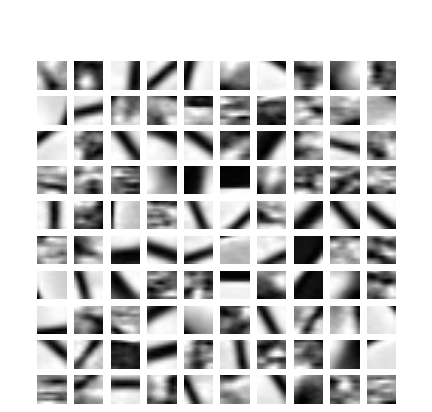
\includegraphics[width=\textwidth]{framework/cluscenters}
						\caption{Learned cluster centers.}
						\label{fig:cluscenters}
					\end{figure}
						
				\column{.45\textwidth} % Left column and width
					\begin{figure}
						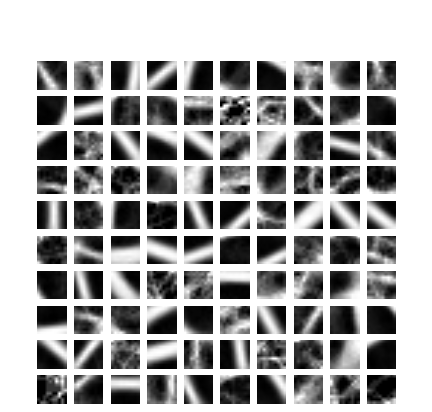
\includegraphics[width=\textwidth]{framework/gtclusters1.png}
						\caption{Segmentation maps for learned clusters.}
						\label{fig:gtclusters}
					\end{figure}					
			\end{columns}


	\end{frame}
	
	\begin{frame}{Parameters}
		There are two important parameters to our patch based Clustering model.
		\begin{itemize}
			\item Patch Size: The size of the patch extracted around each pixel.
			\item K : Number of clusters to be learned.
		\end{itemize}
	\end{frame}
	\begin{frame}{Effect of Patch Size}
		\begin{figure}
			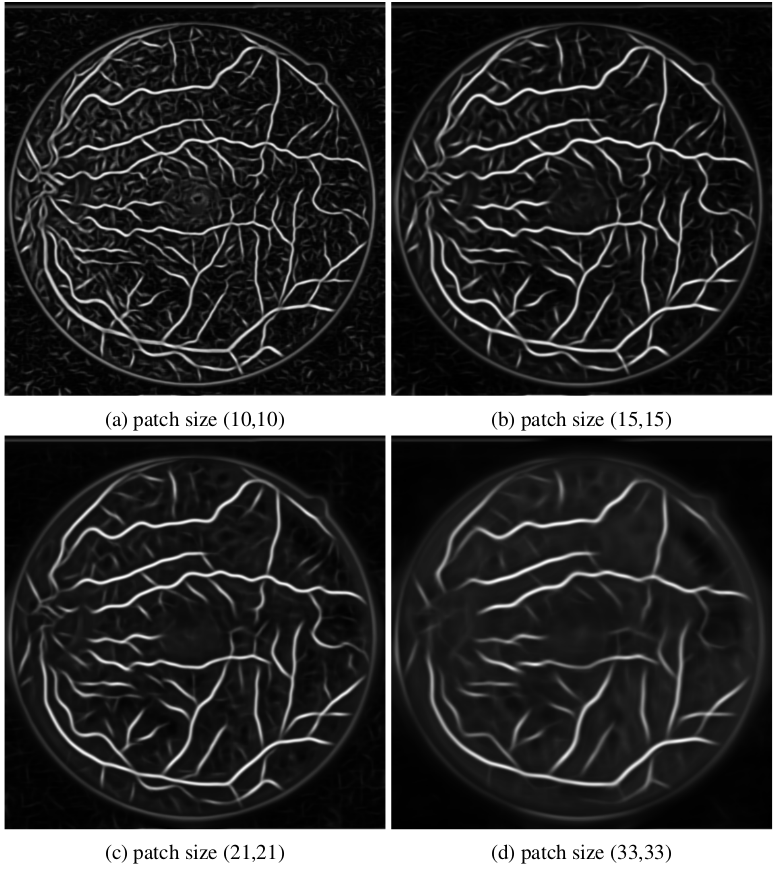
\includegraphics[width=.55\textwidth]{framework/patchsize}

		\end{figure}
	\end{frame}

	\begin{frame}{Effect of Patch Size}
		\begin{figure}
			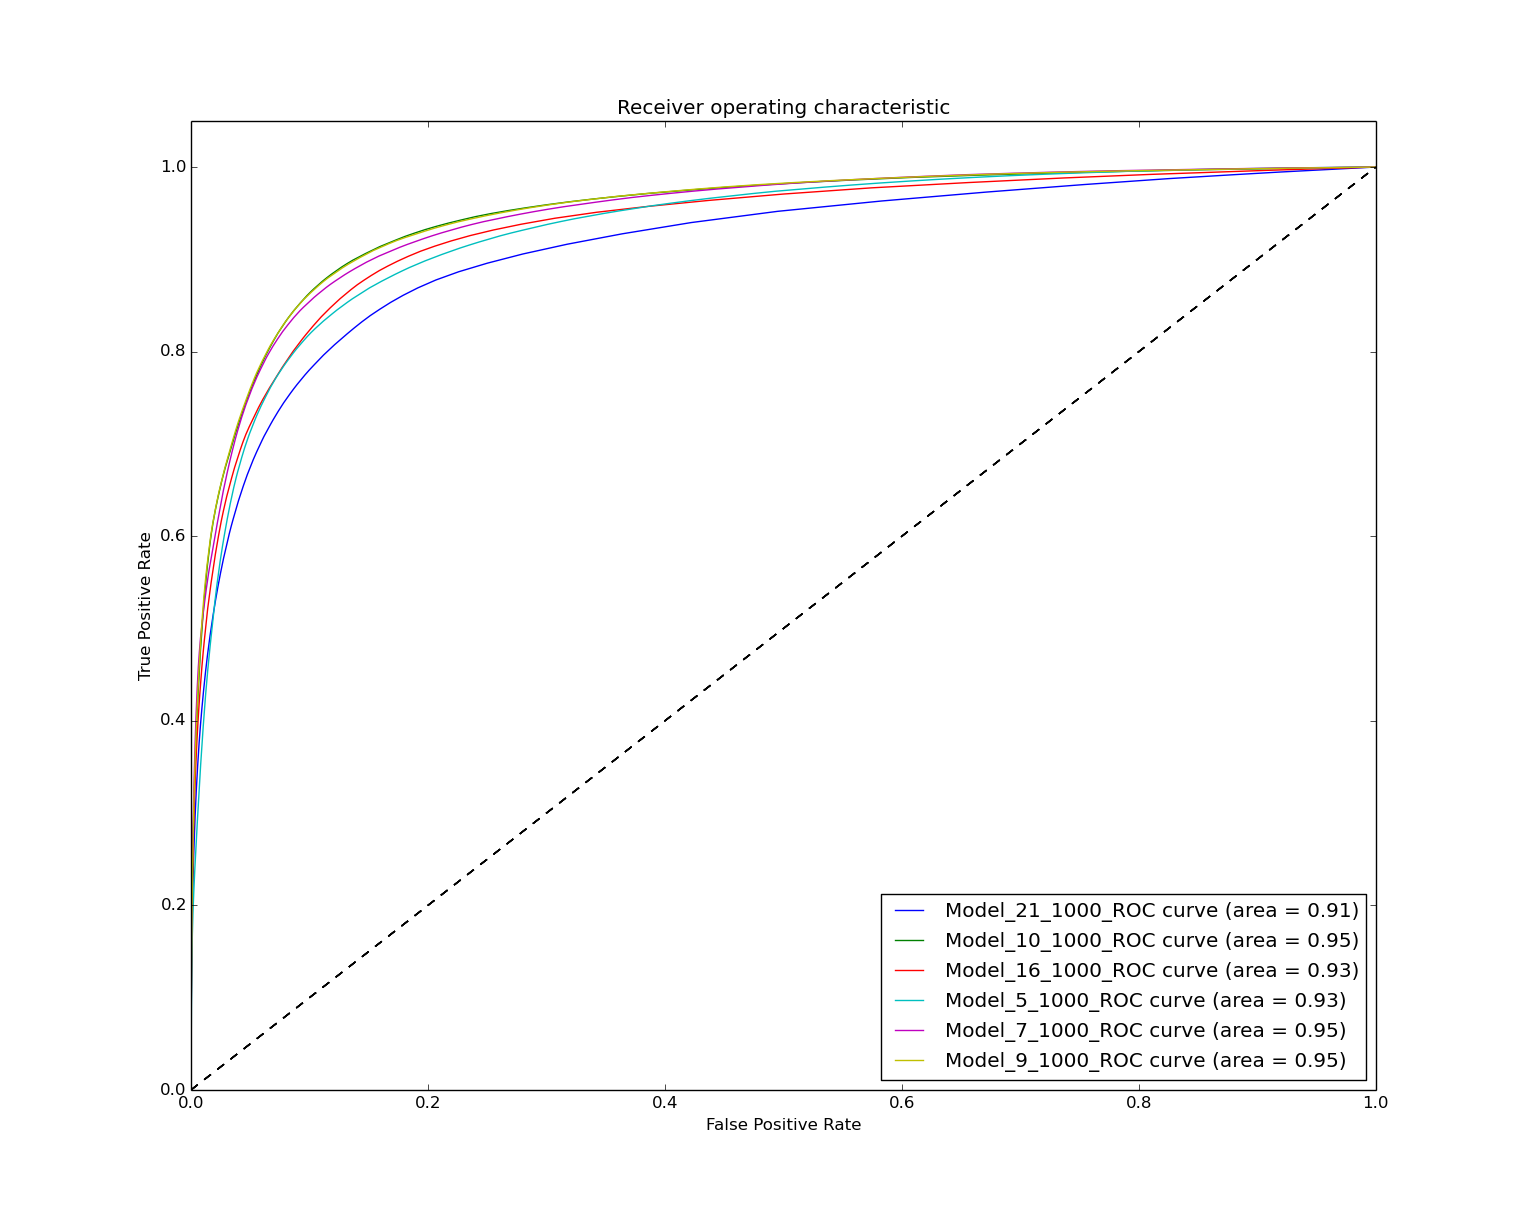
\includegraphics[width=.55\textwidth]{framework/allmod}
			
		\end{figure}
	\end{frame}
	\begin{frame}{Effect of Cluster Size}
		\begin{figure}
			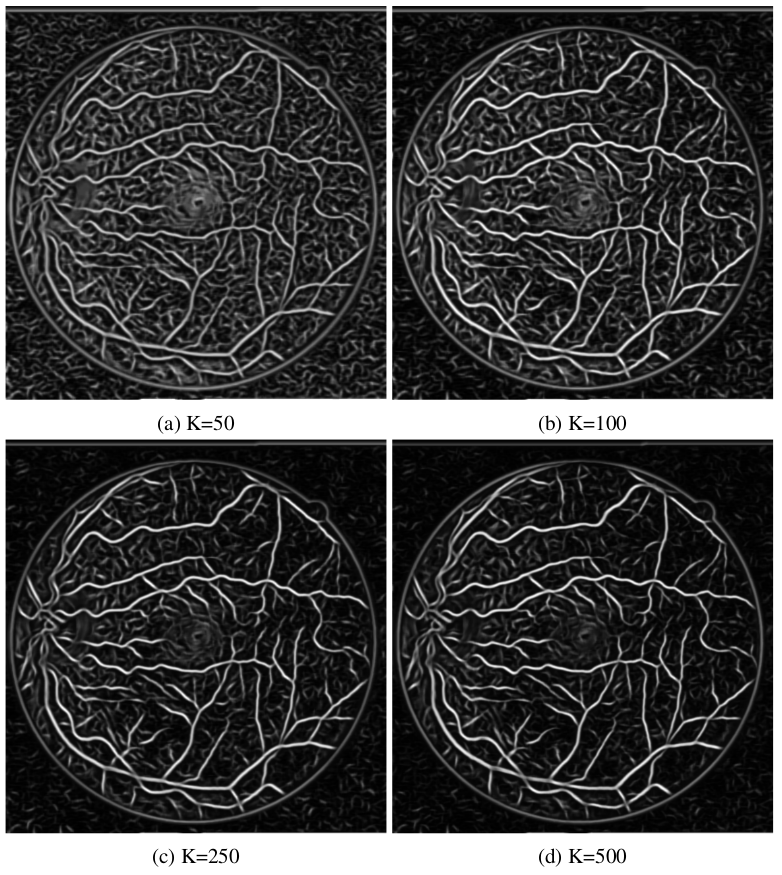
\includegraphics[width=.55\textwidth]{framework/clustersize}
		
		\end{figure}
	\end{frame}
	\begin{frame}{Evaluation on DRIVE dataset}
		We train our model on the DRIVE train set with K=1000 and patch size (10,10) and test on DRIVE test.
		
		We report the results in terms of Area under curve (AUC) for the ROC and PRC curve.
	\end{frame}
	
	\begin{frame}{Receiver operating characteristics}
		\begin{figure}
			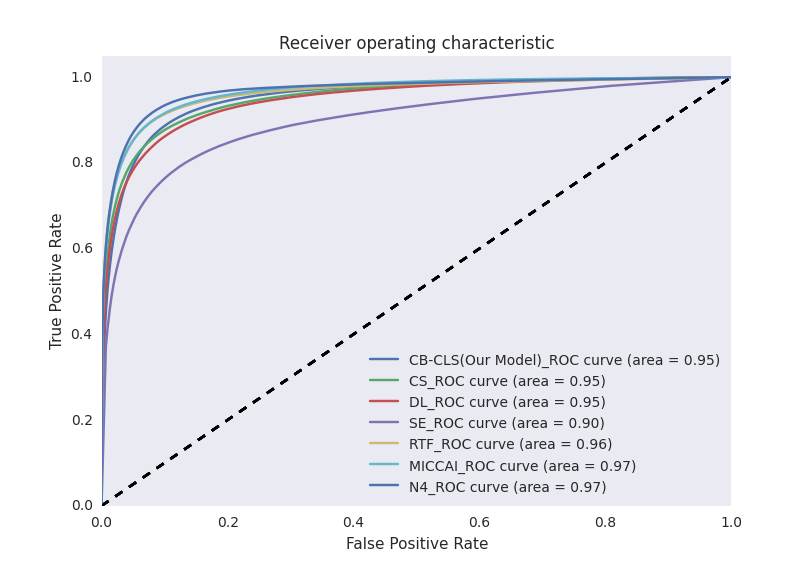
\includegraphics[width=0.9\textwidth]{framework/compareall}			
		\end{figure}
	\end{frame}
	
	\begin{frame}{Precision Recall Curve}
		\begin{figure}
			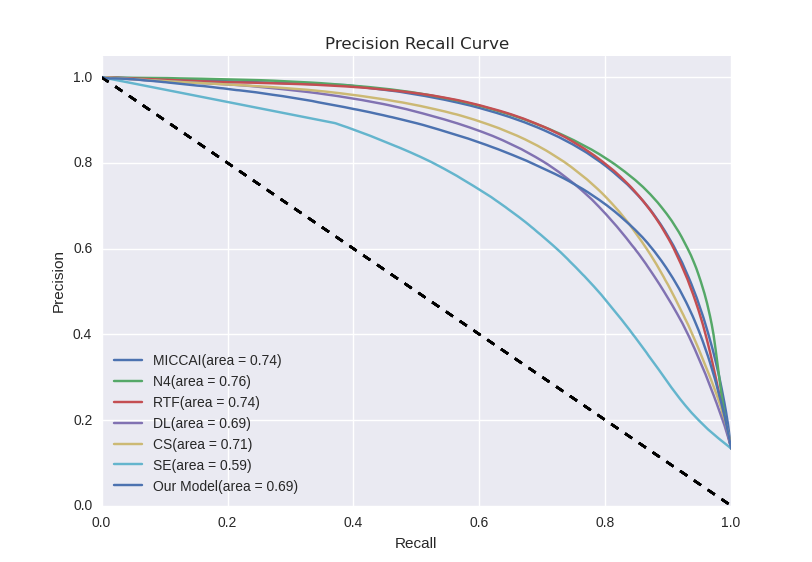
\includegraphics[width=0.9\textwidth]{framework/prcall}			
		\end{figure}
	\end{frame}
	
	\begin{frame}{Best and Worst Case}
		We look into the best case and worst case image prediction on the DRIVE dataset.
		\begin{figure}
			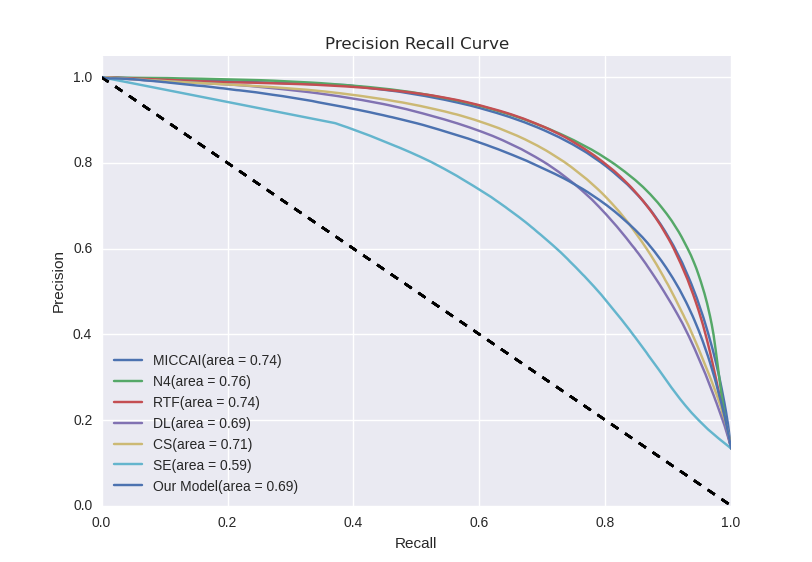
\includegraphics[width=0.9\textwidth]{framework/prcall}			
		\end{figure}
	\end{frame}
\end{document}